\section{Algoritmos de navegação e controle baseados em IA}

Os avanços em algoritmos de controle permitem manobras autônomas sofisticadas com menor intervenção humana e maior resiliência a falhas.
A técnica de aprendizado de máquina (\emph{Machine Learning (ML)}) e redes neurais (\emph{Neural Network (NN)}) são usados para prever dinâmicas orbitais, identificar alvos e planejar trajetórias otimizadas em tempo real.

\subsection{Machine Learning}

Uma das utilidades da utilização do ML é a navegação autônoma de robôs móveis; ela envolve o movimento eficiente de um agente artificial em direção a um destino, evitando colisões e lidando com incertezas ambientais.
Essa área de pesquisa tem sido abordada ao longo das décadas por meio de métodos tradicionais, que combinam um planejamento global de trajetória com controle local de movimento. No entanto, esses métodos apresentam dificuldades ao lidar com ambientes dinâmicos e não estruturados, onde as regras pré-definidas podem não ser suficientes para garantir uma navegação segura e eficiente \cite{xiao2022}.

Devido ao crescimento da pesquisa em \emph{ML}, novas estratégias foram desenvolvidas para aprimorar a navegação autônoma.
As abordagens mais recentes incluem \emph{NN} profundas para o aprendizado ponta a ponta, permitindo que robôs aprendam a relação entre percepção e ação sem a necessidade de um modelo explícito do ambiente, isso faz com que os sistemas se adaptem a diferentes cenários e melhorem sua capacidade de navegação em condições adversas.
O lado negativo dessa técnica é que essas abordagens exigem grandes quantidades de dados e geralmente carecem de interpretabilidade, dificultando a compreensão e correção de erros que possam surgir durante a operação, como explica \cite{xiao2022}.

A utilização de aprendizado de máquina para classificar e prever a periculosidade dos detritos orbitais tem sido explorada como alternativa aos métodos tradicionais baseados exclusivamente em modelos físicos.
Esse método permite analisar grandes volumes de dados obtidos por sensores e sistemas de monitoramento espacial, fornecendo estimativas da ameaça representada por cada detrito com base em sua energia cinética e trajetória.
Os métodos supervisionados de aprendizado têm sido empregados para identificar padrões e categorizar os detritos em diferentes níveis de risco, como baixo, médio e fatal; essa classificação possibilita a criação de estratégias para mitigação de riscos e o desenvolvimento de certificações de segurança para veículos espaciais \cite{sri2024}.

Ainda conforme \cite{sri2024},
O programa de detritos orbitais da NASA tem sido um dos principais referenciais para esse tipo de pesquisa, pois combinam análises físicas com modelagem matemática para prever a distribuição e os impactos dos detritos.
Ao cruzar essas informações com as técnicas de aprendizado de máquina, é possível obter a localização dos fragmentos e a avaliação da probabilidade de colisões.
Dessa forma, a integração entre métodos computacionais e físicos é uma abordagem relevante para melhorar a segurança no ambiente espacial.

\subsection{Neural Network}

Segundo \cite{ke2018}, os modelos de redes neurais profundas (\emph{Deep Neural Network, DNNs}) têm sido utilizadas em diversas aplicações, como visão computacional, processamento de linguagem natural e tradução automática, porém, a execução desses modelos em plataformas computacionais convencionais, baseadas em CPUs é ineficiente devido à alta demanda por processamento paralelo e ao grande consumo de memória.
Para lidar com essas limitações, utilizam-se unidades de processamento gráfico (GPUs).

Ainda como explica \cite{ke2018}, a crescente complexidade das redes neurais e a diversidade de suas arquiteturas impõem desafios para o projeto eficientes.
Cada rede possui características distintas e que influenciam na eficiência do hardware; o que torna inviável tomar uma única abordagem e que atenda a todas as configurações possíveis.
% Nesse contexto, as abordagens de exploração de espaço de projeto (DSE) têm sido adotadas para avaliar diferentes pontos de design e estimar seu impacto no desempenho, consumo de energia e área ocupada pelo circuito. 
% As ferramentas como o \emph{NNest} foram desenvolvidas para facilitar essa análise, permitindo a modelagem de arquiteturas aceleradoras e a comparação de diferentes estratégias de movimentação de dados e ajuste de camadas.

Além da escolha da arquitetura da rede neural, outros fatores afetam a eficiência da execução das NNs, para isso, utilizam-se as estratégias de reutilização de pesos e somas parciais, que podem reduzir a quantidade de operações redundantes.
Métodos de quantização, como redes neurais binárias (BNNs), também vêm sendo explorados para diminuir o consumo de energia e reduzir a complexidade computacional.
% Essas abordagens permitem equilibrar a relação entre precisão do modelo e eficiência computacional, tornando viável a implementação de DNNs em dispositivos embarcados com restrições de potência e área.
A utilização de redes neurais profundas continua a crescer e impulsionam a necessidade de arquiteturas especializadas que ofereçam alto desempenho e baixo consumo de energia.
% O desenvolvimento de novas técnicas de exploração de espaço de projeto e a integração de estratégias de otimização são fundamentais para garantir que essas redes possam ser aplicadas de forma eficiente em diferentes cenários.
A seguir serão expostos exemplos de capacidades autônomas.

\subsection{Boeing Starliner}

A espaçonave \emph{CST-100 Starliner} da Boeing possui capacidades autônomas projetadas para operações de missões espaciais. Abaixo, são detalhados os aspectos principais dessas funcionalidades.

\begin{figure}[H]
    \centering
    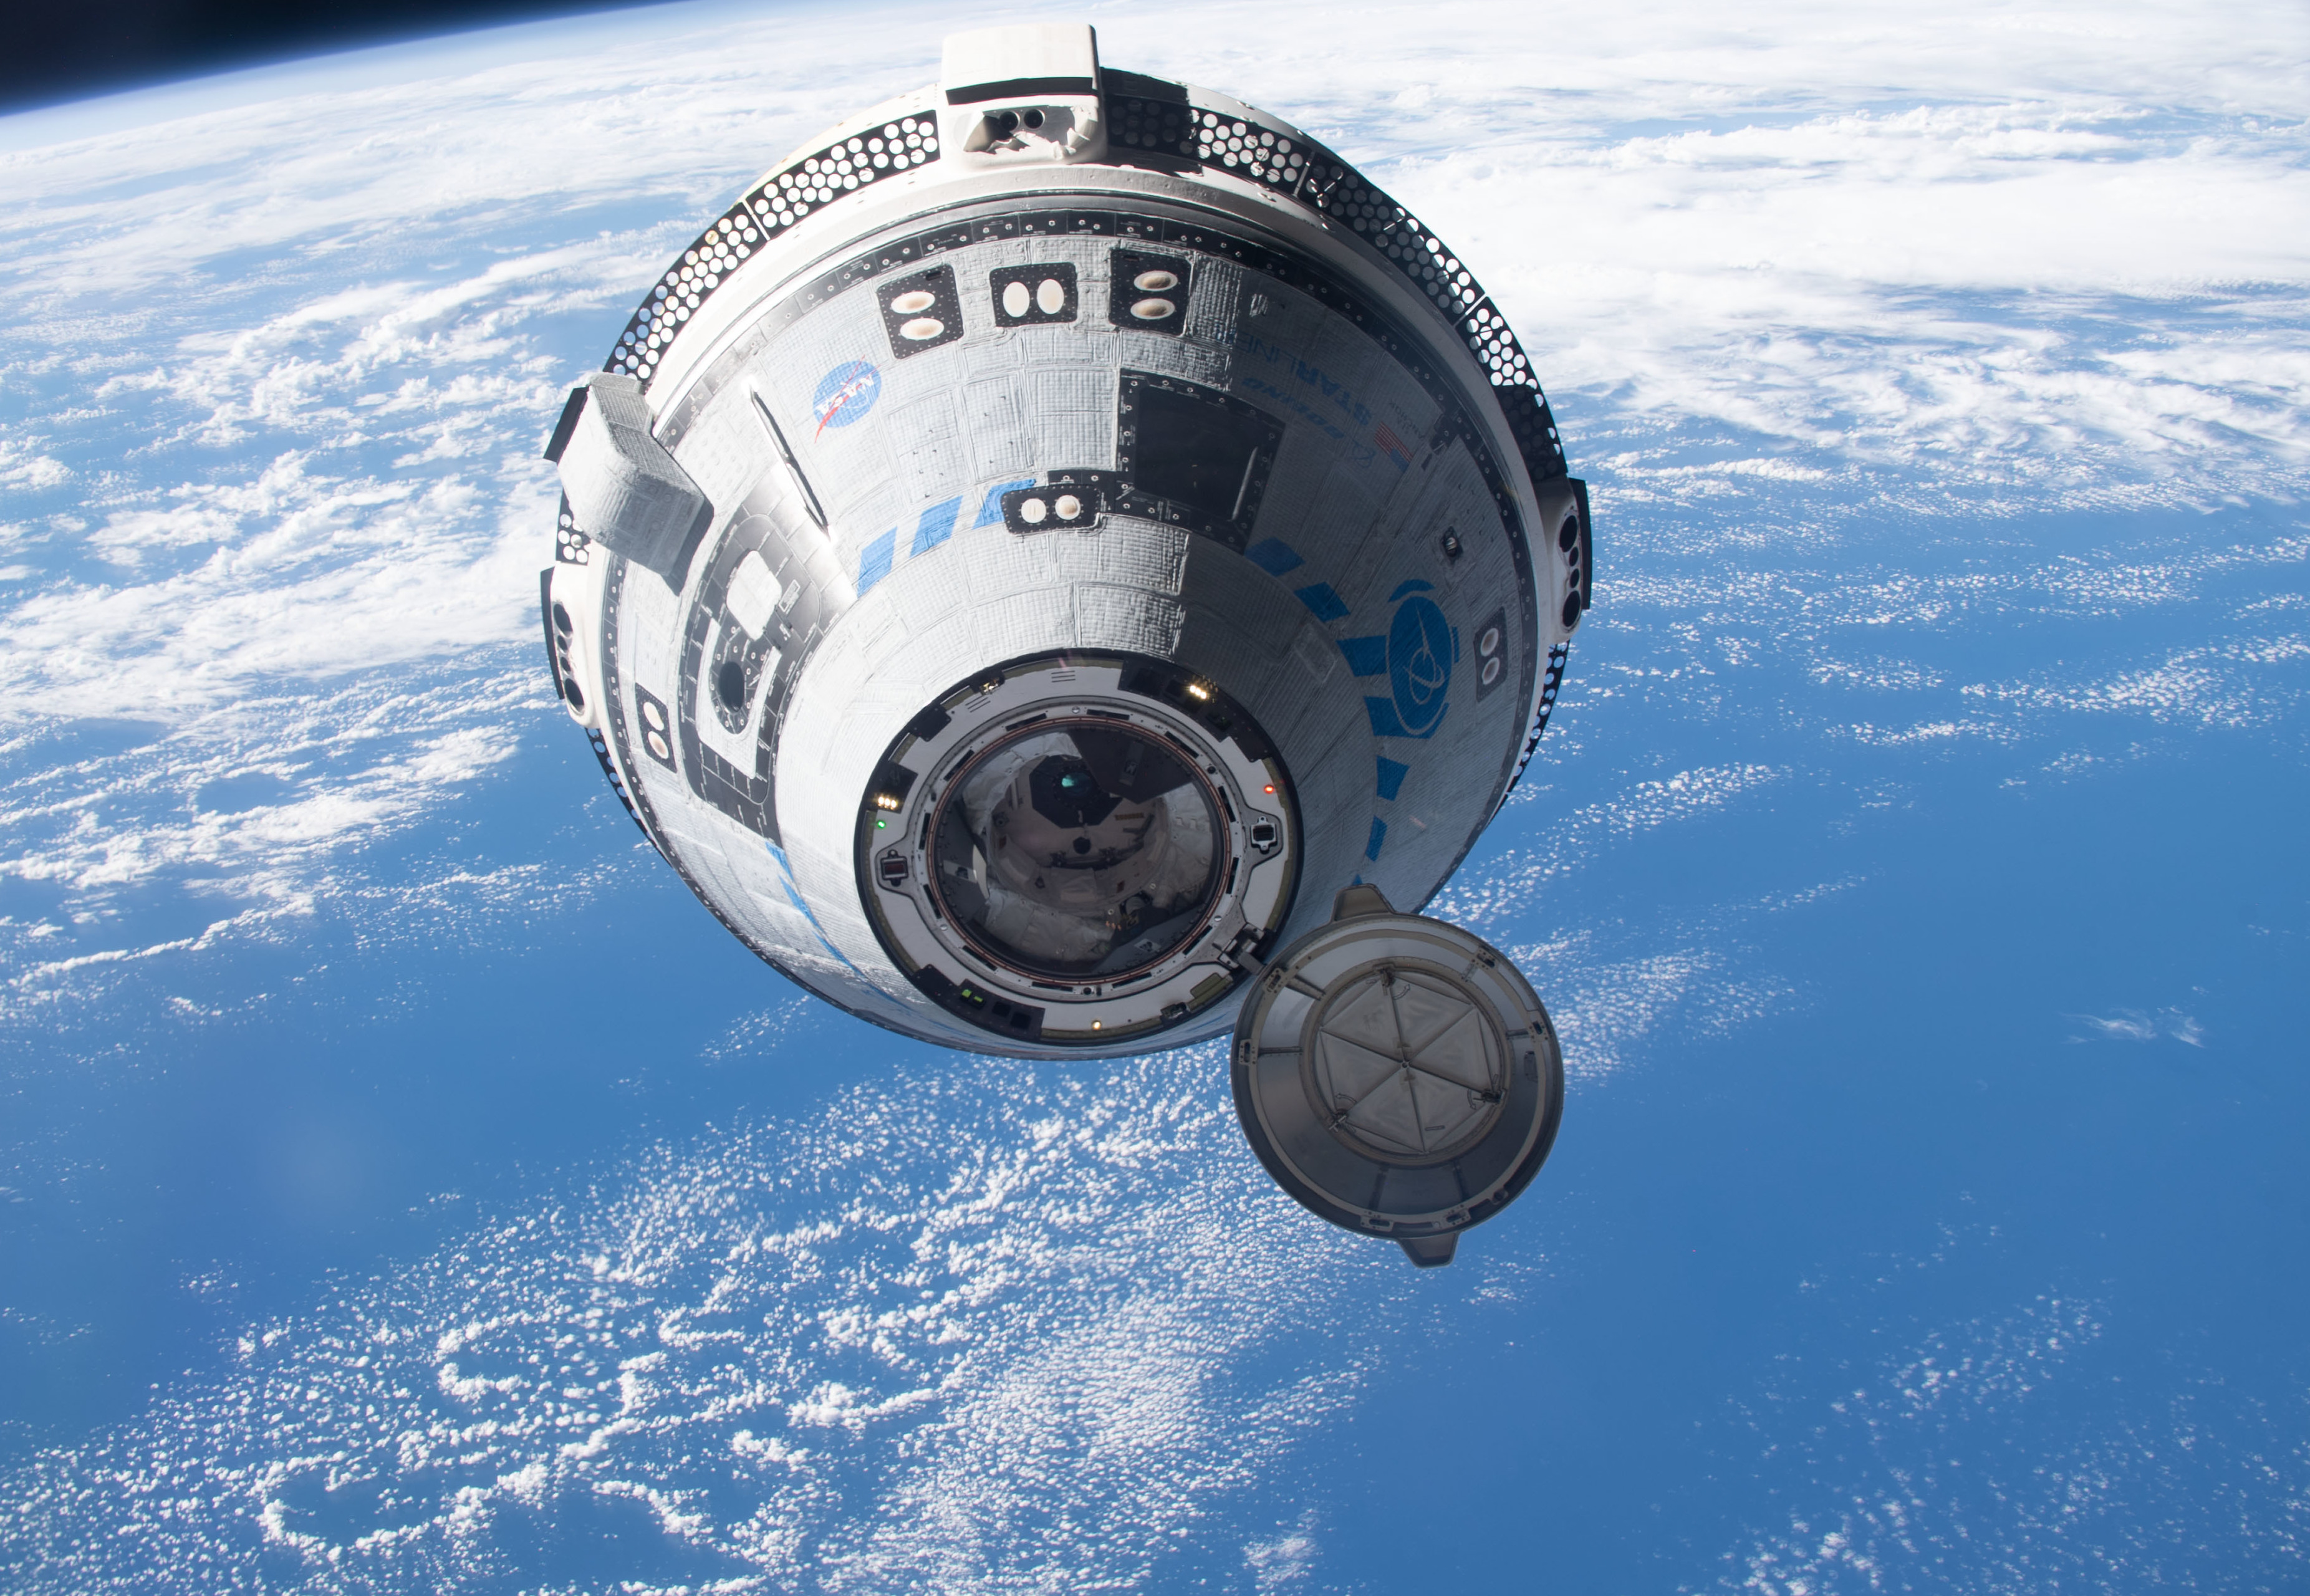
\includegraphics[width=1\linewidth]{1 Introducao/Imagens/Boeing Starliner.jpg}
    \caption{Espaçonave Starliner da Boeing. Fonte: Boeing.}
    \label{fig:BoeingStarliner}
\end{figure}

\subsubsection{Navegação e correção de trajetória autônomas}
A \emph{Starliner} pode realizar navegação com ajustes de curso de forma a não depender de humanos, ou seja, é totalmente independente.
Também é capaz de detectar e corrigir desvios ou erros em sua trajetória durante o voo \cite{boeing2024}.

\subsubsection{Acoplamento automatizado com a ISS}
Por ser equipado com sistemas avançados de sensores e software, a espaçonave pode realizar manobras de RVD/B junto à ISS sem intervenção humana \cite{boeing2024}.

\subsubsection{Capacidade de autodiagnóstico e recuperação}
A espaçonave é equipada com sistemas que monitoram constantemente seu funcionamento e são capazes de detectar anomalias ou falhas.
Em várias situações o \emph{Starliner} pode realizar procedimentos de recuperação de forma automática para resolver falhas identificadas \cite{boeing2024}.

\subsubsection{Operação com e sem tripulação}
Embora tenha capacidade para transportar até setes passageiros na \emph{Starliner}, é possível executar missões autônomas sem tripulação presente, permitindo que o veículo espacial seja empregado em outras funções como o transporte de carga ou testes de sistemas sem depender da intervenção humana \cite{boeing2024}.

\subsubsection{Interface de controle manual para situações de contingência}
Apesar de suas capacidades autônomas avançadas, a \emph{Starliner} está equipada com interfaces que permitem aos astronautas assumir o controle manual da espaçonave quando necessário, sendo assim, quando ocorrer situações imprevistas ou de emergência, a tripulação poderá intervir e conduzir a espaçonave de forma segura \cite{boeing2024}.